%---------------------------------------------------------------------------%
%->> Section 3.3: 面向微服务故障诊断的SOP自动化构建方法
%---------------------------------------------------------------------------%

\section{面向微服务故障诊断的SOP自动化构建方法}

在完成历史故障的统一表示与相似检索之后，系统已经能够从故障指纹库中召回与当前场景相近的历史故障实例。然而，相似实例只能回答“过去发生了什么”，却不能直接回答“当前应如何排查”。对在线诊断而言，真正需要的不只是可供参考的历史案例，还需要一套能够被智能体直接执行的标准操作规程（Standard Operating Procedure，SOP），用于明确排查入口、检查顺序、分支转移条件以及终止判据。

因此，离线知识构建阶段除了构建故障指纹库，还需要进一步把历史故障整理为面向在线诊断的 SOP。这里的关键困难在于：故障实例记录的是故障窗口内的多模态观测结果及最终根因，但并不包含完整的诊断过程；而 SOP 需要显式回答“先检查什么”“依据什么转向”“在什么条件下结束排查”。故障实例与可执行 SOP 之间由此缺少一层能够承接诊断过程的中间表示。围绕这一问题，本文将 SOP 自动化构建组织为如下链路：
\[
\text{故障实例} \rightarrow \text{SOP执行轨迹} \rightarrow \text{决策单元} \rightarrow \text{SOP}.
\]
系统首先围绕历史故障实例执行多轮离线探索，生成带有成功或失败标记的 SOP执行轨迹，把原本缺失的排查步骤、证据依据和路径转移过程显式记录下来；随后从多条轨迹中识别反复出现且能够推动诊断收敛的局部判断，并通过语义对齐和历史统计得到带权决策单元；最后由规则智能体（RuleAgent）结合当前版本 SOP、带权决策单元和代表性轨迹，对 SOP 进行增量更新，形成可供在线诊断直接执行的有向无环图结构。经过这一构建过程，历史故障中的排查经验被逐步整理为能够持续积累和反复调用的结构化诊断知识。

\subsection{SOP构建问题分析与方法设计}

SOP 的价值不在于复述某一次故障，而在于把一次排查中有效的判断依据和路径选择整理为后续同类故障可复用的执行流程。现有运维实践中，这类流程通常由专家根据故障复盘、工单记录和个人经验手工整理，并在系统运行过程中持续更新。这种方式在规模较小、结构相对稳定的系统中仍可工作，但在微服务场景下会迅速暴露出更明显的局限性：

\begin{itemize}
    \item \textbf{排查范围广，人工整理成本高。} 微服务系统通常包含大量服务与复杂依赖关系，一次故障排查往往会跨越多个组件与调用链，人工方式难以稳定覆盖不同场景。
    \item \textbf{系统演化快，流程更新滞后。} 随着部署拓扑、调用关系和故障模式持续变化，人工维护的 SOP 很容易落后于系统实际状态，难以及时反映新的故障传播路径与排查分支。
    \item \textbf{经验环境依赖强，复用性有限。} 人工总结的流程常常绑定具体服务名、实例名或配置细节，在迁移到新环境时仍需重新调整，难以沉淀为稳定的通用诊断知识。
\end{itemize}

在本文的离线阶段中，故障实例主要来自受控的故障注入实验。系统能够获得故障窗口内的指标、日志和调用链路，以及最终确认的故障位置与故障类型。真正的难点不在于收集故障实例，而在于由故障窗口内的观测数据和最终诊断结论推导出合理的排查路径。故障实例能够说明系统在故障窗口内出现了哪些异常、最终根因位于何处，却不能说明排查时先检查了哪些对象、依据什么证据切换方向，以及在何种条件下结束排查。以数据库连接池耗尽为例，一次故障注入实验可以记录支付服务连接错误日志、订单服务响应时延升高、网关请求超时、数据库连接数达到上限，并最终确认根因位于数据库连接池；但这些信息仍不足以还原一条可执行的排查路径。

\begin{figure}[!htbp]
    \centering
    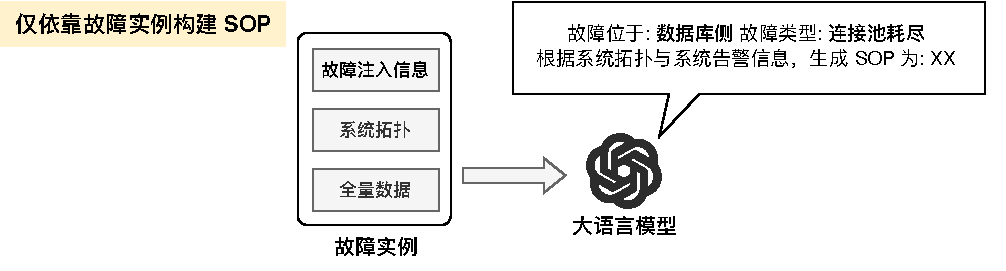
\includegraphics[width=0.82\textwidth]{Figures-Src/Chap3-Methodology/sop-construction-directly/chart.pdf}
    \bicaption{\enspace 由故障实例直接生成SOP的示意}{\enspace Illustration of Direct SOP Generation from Fault Instances}
    \label{fig:sop_direct_generation}
\end{figure}

为了从故障实例中生成可执行的排查路径，一种直观的做法是将故障实例及其相关上下文组织为提示输入，借助大语言模型直接生成 SOP，如图\ref{fig:sop_direct_generation}所示。但这种方法的主要问题在于，模型获得的仍然只是故障观测和最终诊断结论，而中间的排查步骤并未被显式记录，只能由模型根据结果反向推断。因此，生成得到的流程本质上属于基于结果的事后推断。即便这些步骤在表述上看似连贯，其中的检查顺序、转移条件和终止判据仍缺乏真实诊断过程的执行依据，模型甚至可能将故障传播过程中的伴生现象误判为关键诊断线索。对于需要在线执行的诊断系统，仅依赖这种生成方式，难以获得稳定可靠的 SOP。

\begin{figure}[!htbp]
    \centering
    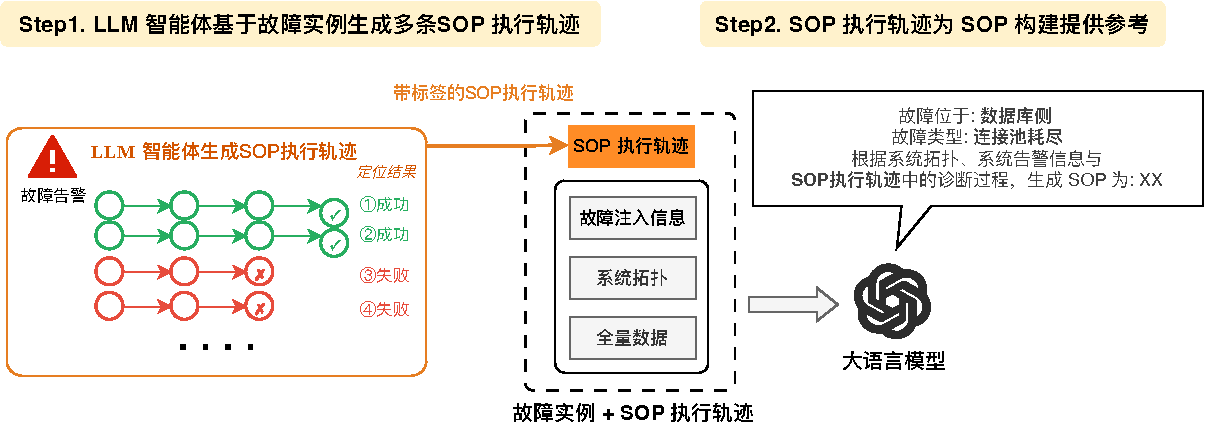
\includegraphics[width=\textwidth]{Figures-Src/Chap3-Methodology/sop-construction-trajectory/chart.pdf}
    \bicaption{\enspace 参照执行轨迹构建SOP的示意}{\enspace Illustration of SOP Construction from Execution Trajectories}
    \label{fig:sop_trajectory_construction}
\end{figure}

为解决仅凭故障观测和最终结论难以直接构建可靠 SOP 的问题，本文在故障实例与最终 SOP 之间引入 \textbf{SOP执行轨迹（SOP Execution Trajectory）} 作为显式中间表示，如图\ref{fig:sop_trajectory_construction}所示。SOP执行轨迹记录离线探索过程中智能体在 SOP 图上的实际执行过程，包括各步检查内容、对应观测证据、路径跳转以及最终诊断结论。因此，SOP 的构建建立在真实执行轨迹之上，而不再依赖模型对中间诊断过程的事后推断。

在引入中间表示之后，还需要进一步确定最终 SOP 的表示形式，使其既能支持后续在线调用，也能支持持续更新。因此面向智能体执行的 SOP 至少应满足以下三项要求：

\begin{enumerate}[label=（\arabic*）]
    \item \textbf{可执行性。} 应显式给出当前需要检查的对象、触发路径转移所依据的证据条件，以及结束排查的判定条件，而不能停留在概括性的自然语言描述上。
    \item \textbf{泛化性。} 不应与某一次故障中的具体服务名、实例名或局部配置直接绑定，否则难以迁移到相似但不完全相同的场景。
    \item \textbf{可增量更新性。} 不应被视为一次性产物，而应能够随着新的执行轨迹持续进行增量更新。
\end{enumerate}

基于上述要求，SOP 不再表示为半结构化的自然语言排障文档，而是借鉴 Think-on-Graph~\cite{sun2024thinkongraph} 中沿图结构逐步推进任务的思路，将 SOP 建模为面向智能体执行的有向无环图（Directed Acyclic Graph，DAG）
\[
G=(V,E),
\]
其中，$V$ 表示诊断节点集合，$E$ 表示节点之间的条件转移关系。Think-on-Graph 将图推理建立在知识图谱中的实体与关系之上，本文则将这一建模思路用于故障诊断流程：图中的节点表示可执行的诊断动作，图中的边表示由观测证据触发的路径转移约束。在线诊断本质上是一个从入口逐步收敛到根因结论的过程。虽然这一过程中可能存在分支选择和路径汇合，但通常不应在既有路径上反复回绕。因此，采用无环结构既有助于智能体稳定执行，也便于后续增量更新。

在该图表示中，节点主要分为入口节点、动作节点和终止节点三类。入口节点对应某类故障排查流程的起点；动作节点表示具体诊断行为，记为
\[
v=\langle \text{Intent}, \text{Entity} \rangle,
\]
其中，$\text{Intent}$ 表示诊断意图，如“检查连接状态”或“验证资源使用率”，$\text{Entity}$ 表示动作作用的目标实体，如“数据库连接池”或“支付服务”；终止节点表示最终识别出的根因结论。边上的条件信息用于刻画节点之间的条件转移关系，即在何种观测结果下进入相应后继节点。基于这种表示，SOP 不再只是对排查流程的静态描述，而成为智能体可直接执行的诊断结构。智能体依据当前观测证据在图上完成判断、执行、观测与转移，并最终收敛到对应的根因结论。


\begin{figure}[!htbp]
    \centering
    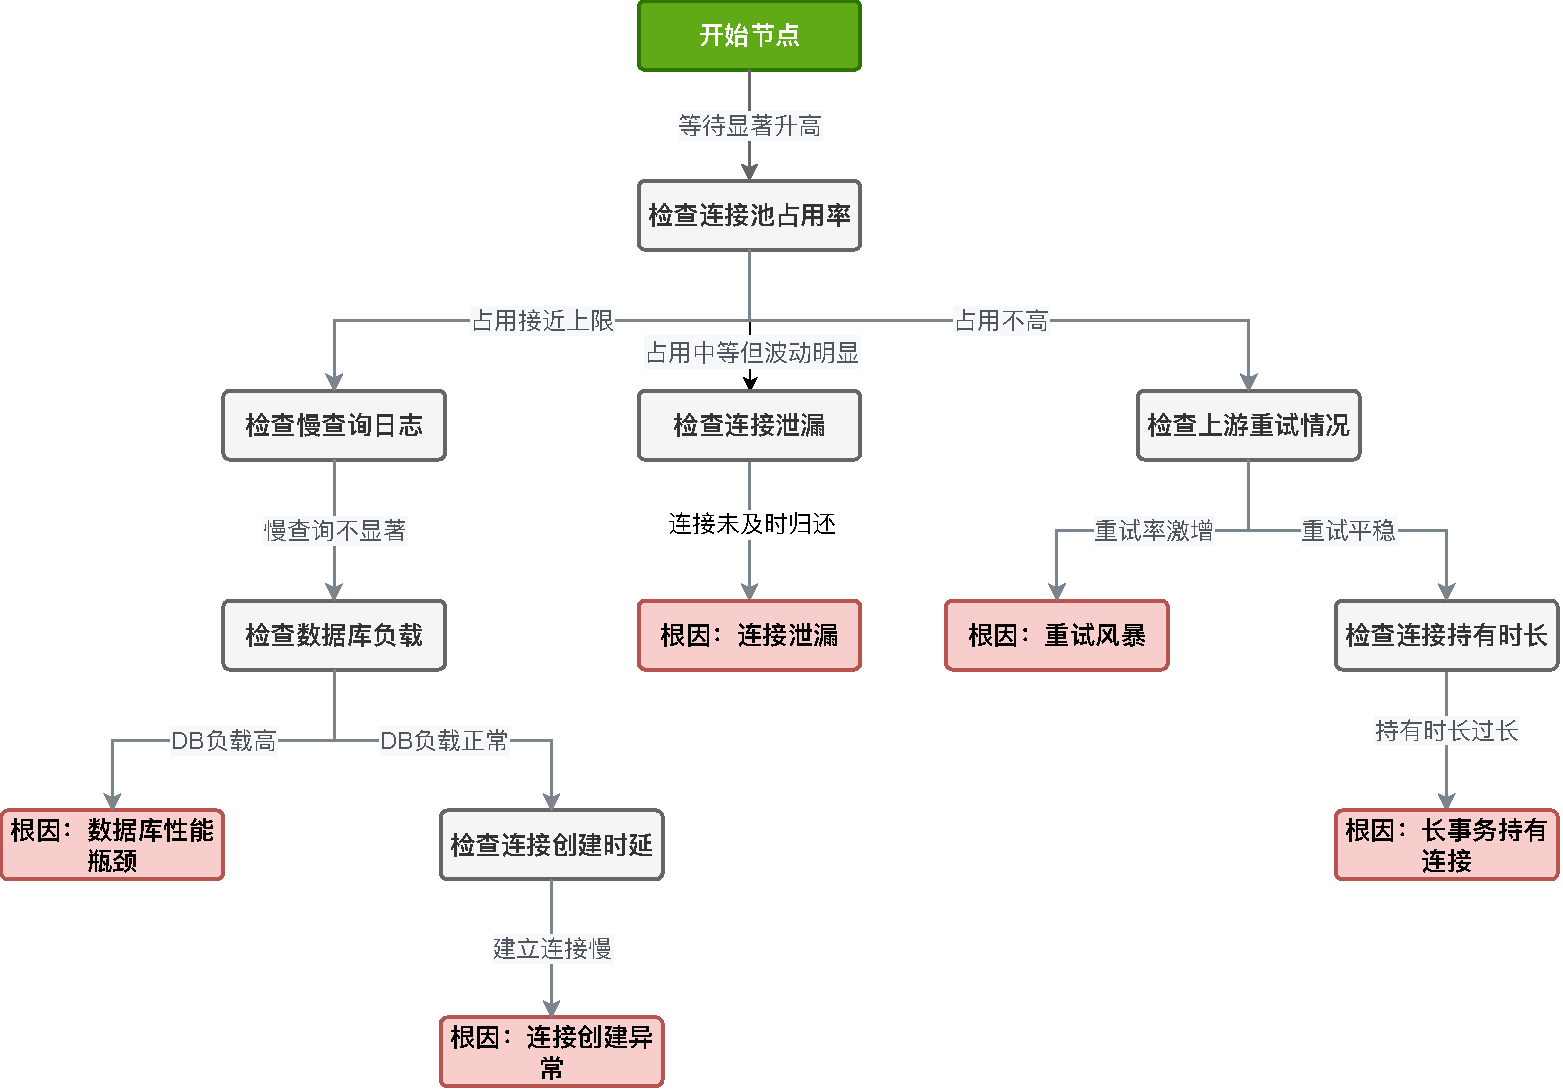
\includegraphics[width=0.75\textwidth]{Figures-Src/Chap3-Methodology/sop-concept-example/chart.pdf}
    \bicaption{\enspace 连接等待显著升高场景的SOP有向无环图示例}{\enspace DAG-based SOP Example for Elevated Connection Wait Time}
    \label{fig:sop_graph_example}
\end{figure}

图\ref{fig:sop_graph_example}给出了数据库场景下的 SOP 有向无环图示例。该图以初始症状为入口，并围绕后续可能的诊断方向组织相应的检查节点。智能体首先检查连接池占用率，再根据“占用接近上限”“占用中等但波动明显”或“占用不高”等不同观测结果，分别进入慢查询日志、连接泄漏、上游重试情况或连接持有时长等后续检查步骤，最终将根因定位为数据库性能瓶颈、连接创建异常、连接泄漏、重试风暴或长事务持有连接等不同结论。该示例说明，SOP 的作用在于将“症状—检查动作—转移条件—根因结论”组织为可执行的诊断流程。

SOP 中的实体不应直接使用历史轨迹中的具体实例名称，而应抽象为可复用的角色化实体。例如，“payment-service-01”应抽象为“上游调用方服务”，“mysql-master-db”应抽象为“数据库连接池组件”。这样既能保留诊断过程中的语义定位信息，又能避免 SOP 绑定于单次实验中的具体实例。至于这些角色化实体如何在在线阶段映射到当前场景中的具体组件，后文将在在线诊断阶段说明。


在此基础上，SOP 的自动化构建可分为三个步骤：

\begin{enumerate}[label=（\arabic*）]
    \item 生成多条 SOP执行轨迹，以显式执行过程还原故障实例中缺失的中间诊断步骤；
    \item 从执行轨迹中提取并对齐决策单元，计算其历史有效性权重；
    \item 在当前版本 SOP 的基础上进行增量整合，形成可执行的有向无环图结构。
\end{enumerate}

经过上述过程，历史故障首先被表示为可比较的诊断执行过程，再进一步整理为可统计、可复用的局部决策结构，最终构造成可直接执行的 SOP 图。

\subsection{故障类型先验的SOP执行轨迹生成}

离线知识构建阶段需要先围绕同一故障实例生成多条可比较的 SOP执行轨迹，用于模拟还原“排查是如何推进的”这一中间过程。本节关注的问题是：\textbf{如何设计离线任务，使智能体能够在历史故障实例上形成可用于后续归纳的诊断执行轨迹。}

一种最直接的做法，是让智能体尽可能模拟真实运维专家的排查方式。具体而言，系统根据故障实例构造模拟的微服务故障环境，智能体只能访问故障窗口内的指标、日志和调用链路等多模态观测数据，并借助相应分析工具逐步缩小可疑范围，最终给出根因结论。系统进一步记录智能体在执行过程中的工具调用与推理过程，作为后续 SOP 构建所需的执行轨迹。由于这种任务设定与真实告警场景最为接近，本文将其称为\textbf{根因定位任务}：智能体不仅需要判断当前故障可能所属的故障类型，还需要继续定位具体的故障组件。

但本文并未直接采用这种任务设定来生成离线轨迹，因为大语言模型在复杂多模态运维数据上的稳定性仍然有限；如果完全以“人类专家视角”独立执行根因定位，智能体往往难以从复杂症状中稳定收敛到真实根因。其直接后果是，正确执行轨迹数量偏少，可用于后续知识沉淀与归纳的正样本不足；而失败轨迹则容易分散到多个无关方向，进一步增加决策单元提取和 SOP 构建的难度。

基于这一考虑，本文将离线任务设定调整为\textbf{故障探索任务}。在该任务中，系统预先给定当前故障的类型标签，探索智能体不再负责判断“这属于哪一类故障”，而是在已知故障类型的前提下，继续围绕该类故障验证可疑组件、传播链路及竞争候选，并记录完整的排查过程。这里引入故障类型先验，并不意味着提前暴露根因位置；其作用在于缩小初始搜索范围，提高有效执行轨迹的比例，并使不同轮次的执行记录能够在同一故障类型内部保持更好的可比性。

设离线故障实例为
\[
\mathcal{I}=(D_{\text{obs}},l^{*},y),
\]
其中，$D_{\text{obs}}$ 表示故障窗口内的可观测数据，$l^{*}$ 表示真实故障位置，$y$ 表示故障类型标签。在轨迹生成阶段，探索智能体可访问的是 $D_{\text{obs}}$、$y$ 和当前版本 SOP $\mathcal{S}$；真实故障位置 $l^{*}$ 对其不可见，仅在轨迹结束后用于判定并标记该轮探索是否成功。

SOP执行轨迹记录的是智能体在 SOP 图上的实际跳转过程。每一步探索都对应一次图上决策：探索智能体根据当前节点、已有证据和故障类型先验判断下一步应检查什么，调用观测能力获取新的指标、日志或调用链路证据，再依据边上的条件决定是否沿现有路径继续推进。若当前 SOP 已经包含足够的节点与边，轨迹就表现为沿既有图结构逐步收敛到根因结论；而在离线构建初期，当前 SOP 往往还是空图，图中既没有可复用节点，也不存在可供满足的出边条件，智能体无法仅依赖现有结构生成轨迹，SOP 结构也难以从空图状态逐步构建。

故障探索任务因此必须允许智能体在必要时扩展图结构。本文将这类操作定义为\textbf{逃逸机制（Escape Mechanism）}。当探索智能体发现当前节点不存在可用出边，或者已有出边的条件与当前证据不匹配，又或者现有 SOP 尚未覆盖当前故障传播路径时，它不再受当前 SOP 已有路径约束，而是依据当前证据自由探索新的诊断方向，并同步构造与这一方向对应的新节点和新边。逃逸本质上是一种在当前 SOP 既有结构之外进行的扩展性探索。它摆脱的是现有路径约束，但探索的目标并不是离开 SOP，而是为 SOP 补入原本尚不存在的节点、边和分支。

在本文设定中，触发逃逸通常对应以下三类情形：

\begin{itemize}
    \item \textbf{当前节点无可用出边。} 现有 SOP 尚未覆盖该状态下的后续诊断动作。
    \item \textbf{已有出边条件与当前证据不匹配。} 现有分支条件不足以解释当前观测，需要构造新的转移关系。
    \item \textbf{需要探索 SOP 尚未覆盖的诊断路径。} 当前故障虽然属于同一类型，但其具体传播方式或可疑对象未被现有 SOP 收录。
\end{itemize}

一次逃逸决策表示为
\[
b_t=\langle v_t^{\mathrm{src}},\rho_t,v_t^{\mathrm{new}},e_t^{\mathrm{new}}\rangle,
\]
其中，$v_t^{\mathrm{src}}$ 表示触发逃逸的源节点，$\rho_t$ 表示触发依据，即当前证据与现有 SOP 不再匹配的原因，$v_t^{\mathrm{new}}$ 表示新建的目标节点，$e_t^{\mathrm{new}}$ 表示连接源节点与目标节点的新边。若该次逃逸最终形成了可验证的根因结论，则说明当前 SOP 在这一类故障下缺少必要的诊断节点、条件边或分支结构；若该次逃逸最终失败，则对应路径只作为失败探索保留在执行轨迹中，而不会直接写入 SOP。一旦某轮探索选择逃逸，后续步骤将沿新生成的路径继续推进；如果在该路径上再次出现“无可用出边”或“条件不匹配”等情形，智能体仍可继续扩展当前逃逸路径。逃逸因此不是一次孤立跳转，而是一条新诊断分支的开始。

故障探索任务由两类智能体协同完成，它们分别负责路径决策和数据观测。

\begin{itemize}
    \item \textbf{探索智能体：} 探索智能体负责在 SOP 图上组织诊断过程。它维护当前节点、已有证据和故障类型先验，决定下一步应检查的对象与诊断意图，并据此选择继续沿现有 SOP 导航、触发逃逸扩展新路径，或在证据满足终止条件时提交根因结论。探索智能体负责基于 SOP 图进行路径决策与过程组织，决定诊断如何推进；而执行过程中实际发生的节点跳转、证据获取和结论提交则会被系统完整记录为 SOP 执行轨迹。
    \item \textbf{观察智能体：} 观察智能体负责与故障实例中的可观测数据交互。它接收探索智能体发送的诊断请求，围绕给定对象与感知域调用指标分析、日志分析和链路查询能力，并将返回结果整理为结构化证据，供探索智能体继续判断。观察智能体不负责决定路径，但它直接决定探索智能体能否获得足够可靠的观测依据。
\end{itemize}


\begin{table}[tbp]
    \centering
    \bicaption{\enspace 探索智能体与观察智能体的工具体系}{\enspace Tool System of the Exploration Agent and Observation Agent}
    \label{tab:dual_agent_tools}
    \renewcommand{\arraystretch}{1.25}
    \fontsize{10pt}{12pt}\selectfont
    \setlength{\tabcolsep}{3pt}
    \begin{tabular*}{\textwidth}{@{\extracolsep{\fill}}>{\centering\arraybackslash}p{1.8cm}>{\centering\arraybackslash}p{2.2cm}>{\raggedright\arraybackslash}p{6.0cm}>{\raggedright\arraybackslash}p{4.0cm}@{}}
        \toprule
        \rowcolor{lightgray!30}
        \textbf{智能体} & \textbf{工具名称} & \textbf{功能描述} & \textbf{关键参数} \\
        \midrule
        \multirow{5}{*}{\textbf{探索智能体}}
        & \texttt{navigate} & 沿 SOP 主链或已有分支跳转 & sop-node-ref \\
        \cline{2-4}
        & \texttt{escape} & 在现有 SOP 无法覆盖时扩展新节点与验证路径 & edge-condition, next-intent \\
        \cline{2-4}
        & \texttt{submit\_message} & 向观察智能体发送查询请求 & prompt \\
        \cline{2-4}
        & \texttt{query\_status} & 查询当前 SOP 状态、节点位置及上下文信息 & current-sop-state \\
        \cline{2-4}
        & \texttt{conclude} & 输出根因结论并汇总关键证据链 & target-component, evidence-chain \\
        \midrule
        \multirow{3}{*}{\textbf{观察智能体}}
        & \texttt{analyze\_metrics} & 当前诊断对象的指标与趋势异常分析 & entity-id \\
        \cline{2-4}
        & \texttt{analyze\_log} & 分析当前诊断对象的日志模式、错误语义及异常事件 & entity-id \\
        \cline{2-4}
        & \texttt{query\_trace} & 查询当前诊断对象的调用链路及上下游 & entity-id \\
        \bottomrule
    \end{tabular*}
    \setlength{\tabcolsep}{6pt}
\end{table}

两类智能体的工具体系如表\ref{tab:dual_agent_tools}所示。探索智能体负责在图上思考、执行跳转、触发逃逸、提交观测请求以及终止任务；观察智能体则负责围绕请求的对象与数据模态，对故障窗口中的指标、日志和调用链路进行具体分析。

在一次故障探索任务中，系统围绕 $(D_{\text{obs}},y,\mathcal{S})$ 重复执行以下过程：探索智能体先根据当前节点、故障类型先验和已有证据确定下一步诊断请求，再通过 \texttt{submit\_message} 将请求发送给观察智能体；观察智能体围绕给定对象调取指标、日志或调用链路证据，并将分析结果返回给探索智能体；探索智能体随后判断应继续沿现有 SOP 图导航，还是触发逃逸扩展新的路径，并在证据充分时提交根因结论。对于执行过程中实际发生的动作、证据获取、节点跳转和结论提交，系统都会统一记录。由此形成的执行记录不仅包含工具调用顺序，也完整保留了智能体在 SOP 图上推进、切换和扩展诊断路径的过程。

系统将第 $r$ 轮探索过程中实际发生的动作、证据、节点跳转、逃逸决策和结论判定统一记录为一条 SOP 执行轨迹，记为
\[
\tau_r=(\mathcal{A}_r,\mathcal{E}_r,\mathcal{P}_r,\mathcal{B}_r,\mathcal{J}_r,\ell_r),
\]
其中，$\mathcal{A}_r$ 表示诊断动作序列，$\mathcal{E}_r$ 表示对应的证据观察，$\mathcal{P}_r$ 表示节点跳转记录，既包括沿现有 SOP 边的导航跳转，也包括由逃逸产生的新边跳转；$\mathcal{B}_r$ 表示逃逸决策记录，其中显式保留源节点、触发依据、新建节点和新建边；$\mathcal{J}_r$ 表示结论判定记录，$\ell_r$ 表示依据真实故障位置 $l^{*}$ 赋予的轨迹标签。

\begin{figure}[tbp]
    \centering
    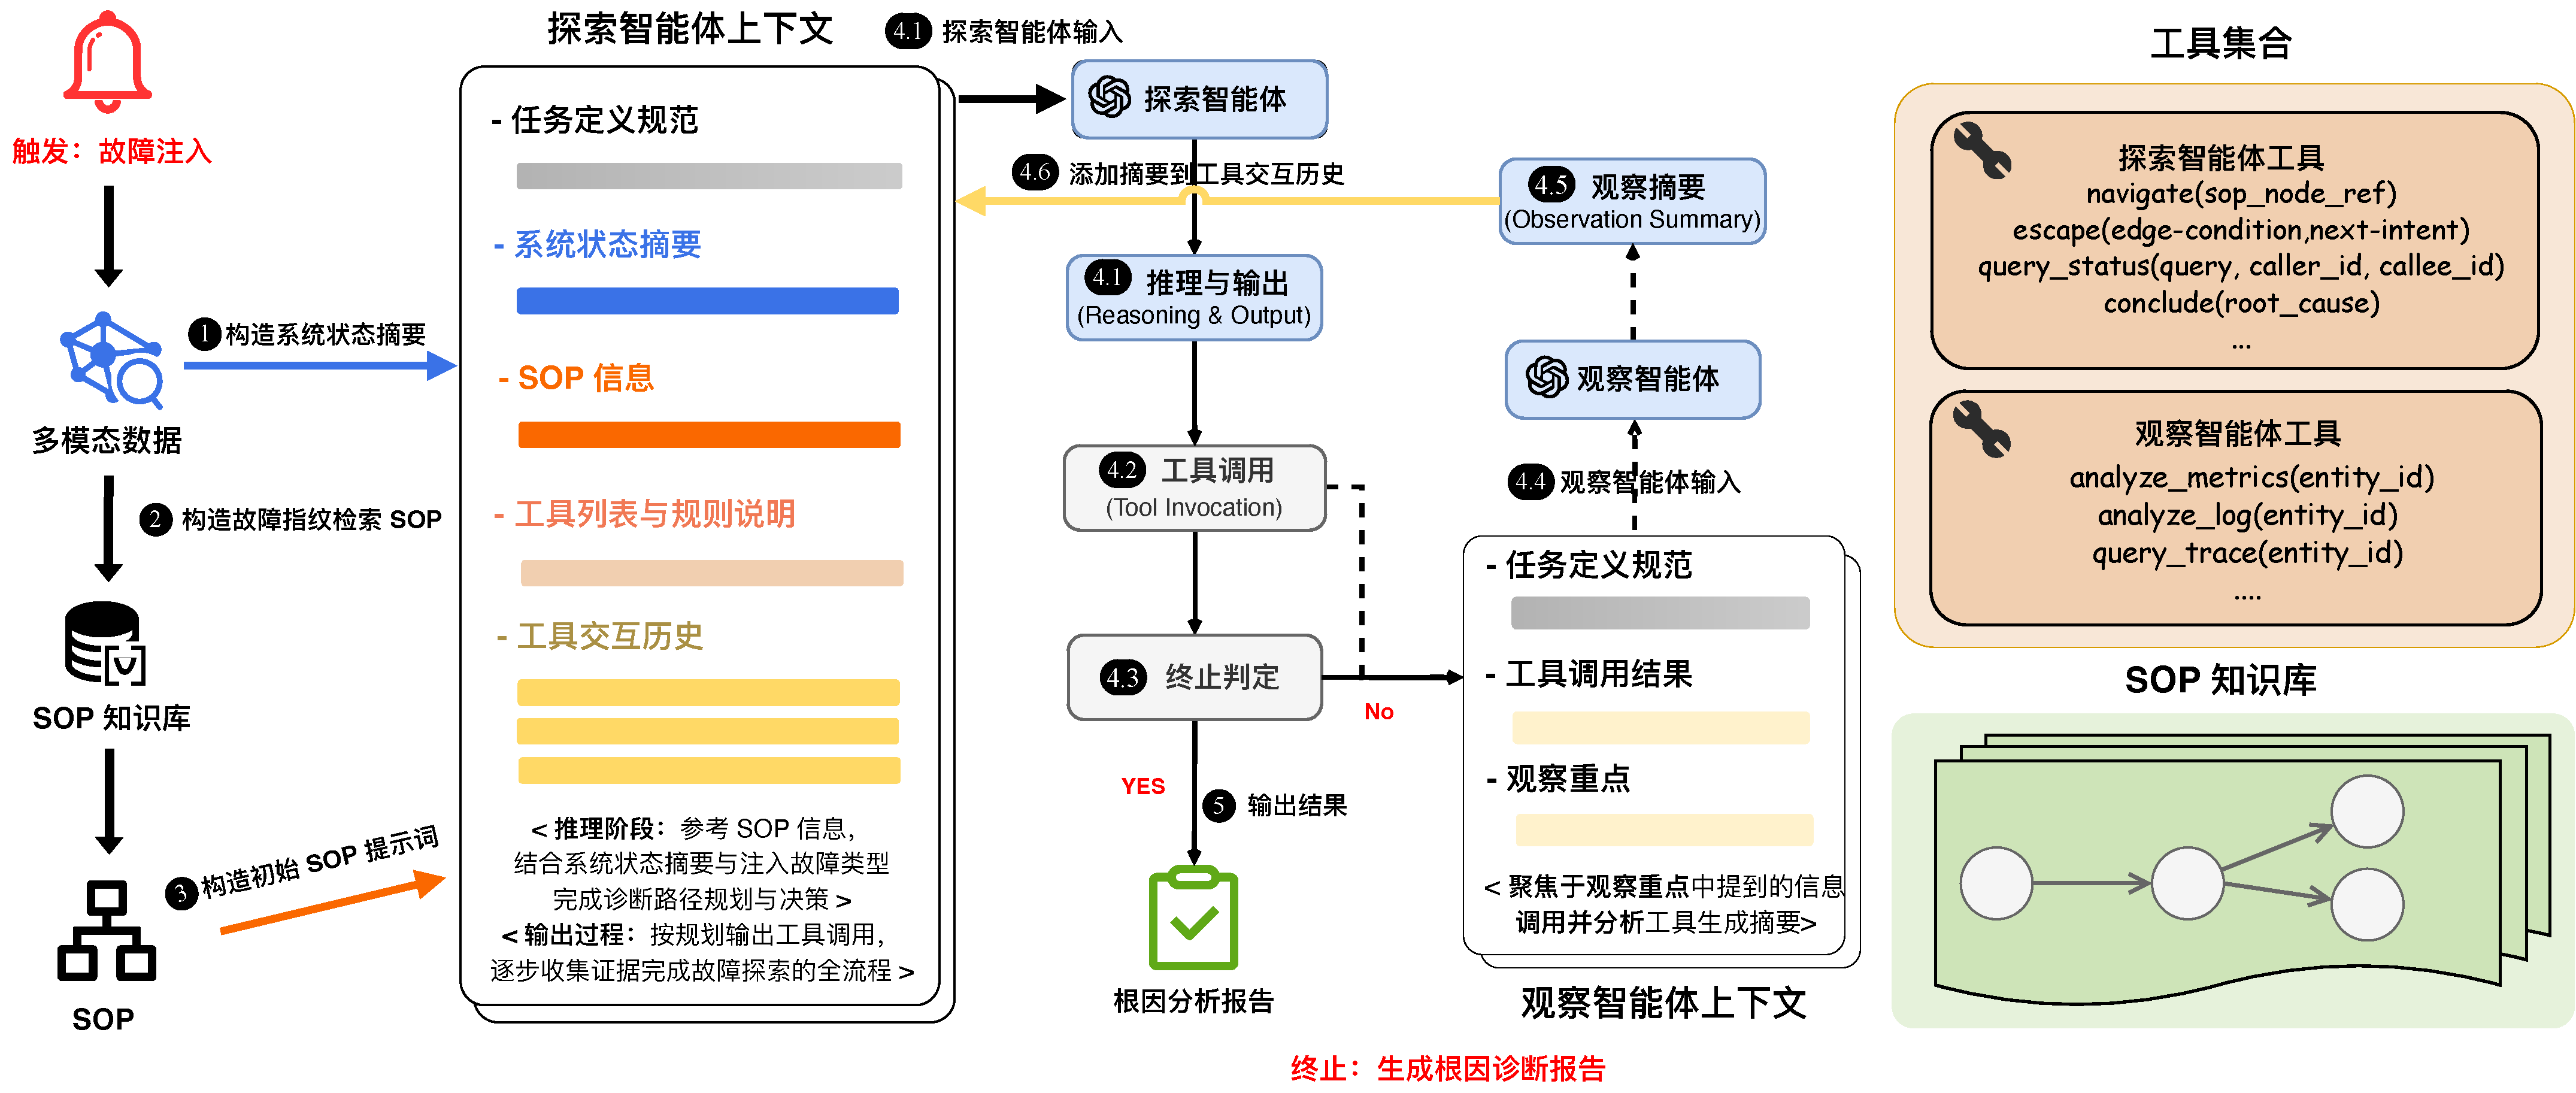
\includegraphics[width=\textwidth]{Figures-Src/Chap3-Methodology/exploration-agent-interaction/chart.pdf}
    \bicaption{\enspace 探索智能体与观察智能体的协作流程}{\enspace Collaboration Flow of the Exploration Agent and Observation Agent}
    \label{fig:exploration_interaction_arch}
\end{figure}

图\ref{fig:exploration_interaction_arch}给出了探索智能体与观察智能体的协作过程。系统提供状态查询、多模态证据分析、导航、逃逸和结论提交五类操作，分别对应 \texttt{query\_status}、\texttt{analyze\_metrics}、\texttt{analyze\_log}、\texttt{query\_trace}、\texttt{navigate}、\texttt{escape} 和 \texttt{conclude}。其中，\texttt{navigate} 对应沿现有 SOP 出边推进，\texttt{escape} 对应在当前图结构无法继续推进时创建新的节点和边。

\begin{figure}[tbp]
    \centering
    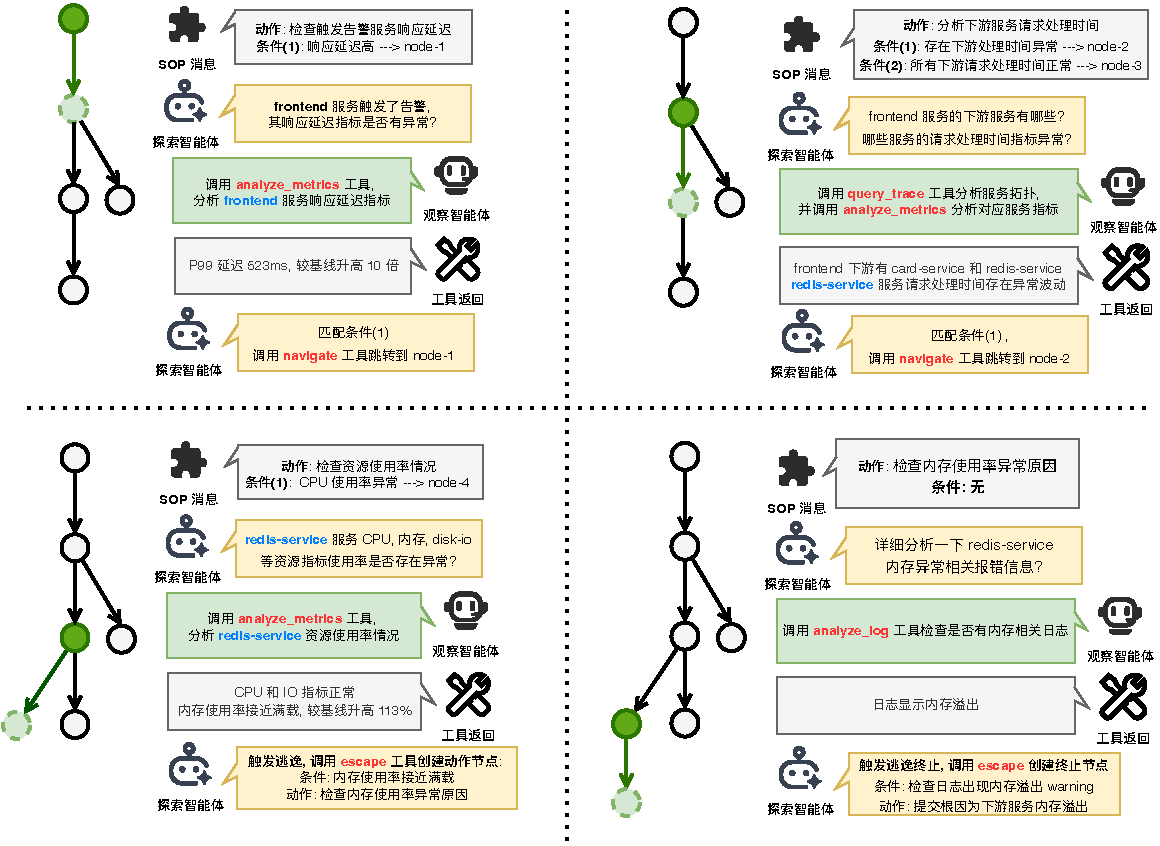
\includegraphics[width=\textwidth]{Figures-Src/Chap3-Methodology/exploration-agent-example/chart.pdf}
    \bicaption{\enspace 探索智能体与观察智能体的协同示例}{\enspace One Collaboration Example of the Exploration Agent and Observation Agent}
    \label{fig:exploration_interaction_example}
\end{figure}

图\ref{fig:exploration_interaction_example}进一步展示了一次具体协同示例：探索智能体根据当前待验证对象调用观察智能体分析指标与日志，并根据返回证据决定继续沿既有路径推进，还是通过逃逸机制生成新的目标节点与转移边。系统以故障实例 $\mathcal{I}=(D_{\text{obs}},l^{*},y)$ 为输入，在当前版本 SOP 的约束下反复执行候选对象初始化、证据收集、路径跳转、逃逸扩展和结论判定等操作。这里的 \texttt{conclude} 仅表示探索智能体提交当前轮次的根因判断，轨迹是否真正成功仍由真实故障位置 $l^{*}$ 在轮次结束后统一标注。

为避免智能体仅凭某个显著异常就过早结束排查，轨迹终止时采用双重结论判定准则：一方面，轨迹中必须形成从表面症状到候选根因的主证据链，即最终结论需要建立在连续、可追溯、能够相互支撑的证据序列之上；另一方面，对于与当前根因判断高度相关的竞争候选，还需要完成排除性验证并给出相应证据。例如，当观察到数据库时延升高时，智能体不能直接将数据库判为根因，还需要进一步排除网络抖动或缓存失效等可能的传播来源。只有当主证据链成立且关键竞争候选被排除后，当前轨迹才被视为满足结论判定条件。

在同一故障场景下，系统会执行多轮相互独立的探索，以获得一组可比较的 SOP执行轨迹。按“是否发生逃逸”和“是否成功定位”两个维度，轨迹被划分为四类：

\begin{enumerate}[label=（\arabic*）]
    \item \textbf{非逃逸成功轨迹。} 现有 SOP 图中已经存在足够的节点、边和条件约束，智能体无需生成新路径即可定位到真实根因，可作为保留主路径的依据。
    \item \textbf{逃逸成功轨迹。} 智能体在某一步找不到可用出边，或现有边条件无法匹配当前证据，因而通过逃逸生成了新的节点和边，并最终成功定位根因。这类轨迹是补全 SOP 新分支的直接来源。
    \item \textbf{非逃逸失败轨迹。} 智能体沿现有主路径推进后仍无法定位根因，表明其中某个条件、节点设计或已有分支结构尚不准确。
    \item \textbf{逃逸失败轨迹。} 智能体虽然生成了新的候选路径，但该路径最终未能形成可验证结论，因此只能作为失败样本保留，而不应直接写入 SOP。
\end{enumerate}

本阶段最终输出的是多条带标签的 SOP 执行轨迹，每条轨迹同时包含动作序列、证据观察、节点跳转、逃逸决策、结论判定以及成败标记。这些轨迹构成后续决策单元提取与权重计算的直接输入；系统同时保留该故障实例对应的故障指纹，用于后续故障簇与 SOP 的绑定。

\subsection{决策单元提取与权重计算}

上一阶段得到的多条 SOP执行轨迹记录了诊断过程中实际发生的检查动作、证据引用、条件转移和阶段性结论，但轨迹本身仍属于过程性记录，尚不能直接纳入 SOP。其原因在于：同一诊断动作在不同轨迹中常以不同表述出现；部分轨迹片段仅对应一次性试探或冗余验证；个别分支虽然被执行，但并未对根因定位产生实质作用。若直接保留整条轨迹，容易使更新后的 SOP 出现节点重复、分支膨胀以及无效步骤混入等问题。

为此，本文先将轨迹拆分为可复用的基本单元，再据此完成后续的 SOP 组织。本文将该基本单元定义为决策单元（Decision Unit），记为
\begin{equation}
u=\langle n,e\rangle,
\end{equation}
其中，节点 $n$ 表示当前诊断动作，
\begin{equation}
n=\langle \text{Intent},\text{Entity}\rangle,
\end{equation}
边 $e$ 表示由条件触发的转移关系，
\begin{equation}
e=\langle \text{Condition},\text{Next}\rangle.
\end{equation}
其中，$\text{Intent}$ 表示当前步骤的检查意图，$\text{Entity}$ 表示被检查对象，$\text{Condition}$ 表示触发转移的判断条件，$\text{Next}$ 表示满足条件后的后继节点。这样，一个决策单元同时刻画了“当前检查什么”以及“在何种条件下转向何处”两个信息。例如，“检查数据库连接池状态”与“若连接数达到上限，则转向检查连接泄漏”可共同表示为一个完整的决策单元。

设 SOP执行轨迹集合为 $\mathcal{T}=\{\tau_1,\tau_2,\ldots,\tau_N\}$，则每条轨迹首先被拆分为决策单元序列
\begin{equation}
\mathcal{U}_{\tau_i}=\textsc{SplitUnits}(\tau_i),
\end{equation}
并汇总得到候选决策单元集合
\begin{equation}
\mathcal{U}=\bigcup_{i=1}^{N}\mathcal{U}_{\tau_i}.
\end{equation}
这里，$\mathcal{U}$ 同时包含沿既有 SOP 路径抽取的决策单元，以及由逃逸机制生成并在后续执行中被验证的新增决策单元。

为消除表述差异带来的重复记载，本文将每个决策单元统一编码为文本序列
\begin{equation}
c(u)=\text{Intent}\oplus \text{Entity}\oplus \text{Condition},
\end{equation}
并利用语义嵌入模型将其映射到向量空间
\begin{equation}
\mathbf{z}_{u}=f_{\mathrm{emb}}\big(c(u)\big).
\end{equation}
在此基础上，对向量集合 $\{\mathbf{z}_{u}\mid u\in\mathcal{U}\}$ 进行基于密度的聚类，得到语义一致的决策单元簇
\begin{equation}
\mathcal{C}=\{C_{1},C_{2},\ldots,C_{M}\}=\textsc{DBSCAN}\big(\{\mathbf{z}_{u}\}\big).
\end{equation}
每个簇 $C_j$ 对应一类语义相近、但原始表述可能不同的决策单元。

完成语义对齐后，本文进一步从历史轨迹中评估各决策单元簇的保留价值。考虑到 SOP 更新的目标是保留能够稳定支持根因定位的步骤，本文从互信息、方向性、拓扑位置和逃逸有效性四个维度对每个簇 $C_j$ 进行加权。

\paragraph{1) 互信息（Mutual Information, MI）}
互信息用于度量决策单元簇 $C_j$ 与诊断成功之间的统计关联。设
\begin{equation}
x_{\tau,j}=\mathbb{I}(C_j \cap \mathcal{U}_{\tau}\neq \varnothing),
\end{equation}
表示轨迹 $\tau$ 中是否出现过簇 $C_j$，$y_{\tau}\in\{0,1\}$ 表示该轨迹是否成功定位根因，则
\begin{equation}
\mathrm{MI}_{j}=\sum_{x\in\{0,1\}}\sum_{y\in\{0,1\}}p_{j}(x,y)\log \frac{p_{j}(x,y)}{p_{j}(x)\,p(y)}.
\end{equation}
$\mathrm{MI}_{j}$ 越大，说明该决策单元与成功诊断的关联越强，更适合作为稳定步骤写入 SOP。

\paragraph{2) 方向因子（Direction Factor, DF）}
方向因子用于衡量某一决策单元在执行后是使诊断更接近根因，还是使路径偏离主线。记 $O_j$ 为簇 $C_j$ 在全部轨迹中的出现位置集合。对于任一出现位置 $(\tau,t)\in O_j$，设 $d^-_{\tau,t}$ 表示执行该单元之前当前节点到终止节点的剩余步数，$d^+_{\tau,t}$ 表示执行该单元并完成转移后到终止节点的剩余步数，则
\begin{equation}
\mathrm{DF}_{j}=\frac{1}{|O_j|}\sum_{(\tau,t)\in O_j}\frac{d^-_{\tau,t}-d^+_{\tau,t}}{d^-_{\tau,t}+1}.
\end{equation}
当 $\mathrm{DF}_{j}>0$ 时，说明该决策单元总体上推动路径朝终止节点收敛；当 $\mathrm{DF}_{j}<0$ 时，说明该单元更常出现在偏离根因的路径中。

\paragraph{3) 拓扑距离（Topology Distance, TD）}
拓扑距离用于描述决策单元在一条有效诊断路径中的相对位置。对于出现位置 $(\tau,t)\in O_j$，设 $L_{\tau}$ 为轨迹 $\tau$ 的总步数，$\ell_{\tau,t}$ 为该位置到轨迹终止节点的剩余步数，则定义
\begin{equation}
\mathrm{TD}_{j}=1-\frac{1}{|O_j|}\sum_{(\tau,t)\in O_j}\frac{\ell_{\tau,t}}{L_{\tau}}.
\end{equation}
$\mathrm{TD}_{j}$ 越大，说明该决策单元越接近诊断收敛位置。该指标可用于区分早期的广泛筛查步骤与后期具有更强定位作用的关键步骤。

\paragraph{4) 逃逸有效性（Escape Validity, EV）}
逃逸有效性用于衡量决策单元在逃逸路径中的实际贡献。记 $O_j^{\mathrm{esc}}\subseteq O_j$ 为簇 $C_j$ 在逃逸路径中的全部出现位置集合，则
\begin{equation}
\mathrm{EV}_{j}=
\frac{\sum_{(\tau,t)\in O_j^{\mathrm{esc}}} y_{\tau}}
{|O_j^{\mathrm{esc}}|+\varepsilon},
\end{equation}
其中，$\varepsilon$ 为防止分母为零的平滑项。当 $\mathrm{EV}_{j}$ 较高时，说明该决策单元虽然并非总来自既有 SOP 主路径，但在历史逃逸过程中多次参与了有效收敛，因而具有保留价值。

由于四个指标的量纲不同，本文先对各指标进行归一化处理。对于任一指标 $s\in\{\mathrm{MI},\mathrm{DF},\mathrm{TD},\mathrm{EV}\}$，记其归一化结果为
\begin{equation}
\widehat{s}_{j}=
\frac{s_{j}-\min_{k}s_{k}}
{\max_{k}s_{k}-\min_{k}s_{k}+\varepsilon}.
\end{equation}
在此基础上，决策单元簇 $C_j$ 的综合权重定义为
\begin{equation}
w_j=\alpha_{1}\widehat{\mathrm{MI}}_{j}
+\alpha_{2}\widehat{\mathrm{DF}}_{j}
+\alpha_{3}\widehat{\mathrm{TD}}_{j}
+\alpha_{4}\widehat{\mathrm{EV}}_{j},
\qquad
\sum_{m=1}^{4}\alpha_m=1.
\end{equation}
其中，$\alpha_m$ 为各指标的组合系数。$w_j$ 并不直接决定某一决策单元是否被保留，而是为后续 SOP 增量更新提供排序依据：当多个候选步骤具有相似语义时，权重更高者优先进入 SOP 结构。

综上，经过拆分、对齐与加权后，系统得到带权决策单元集合
\begin{equation}
\mathcal{U}^{w}=\{u^{w}_{1},u^{w}_{2},\ldots,u^{w}_{M}\}.
\end{equation}
集合中的每个元素均包含统一语义标识、诊断意图、目标实体、触发条件及其综合权重。相较于原始轨迹，带权决策单元已经从过程性记录转化为可直接参与 SOP 更新的结构化知识，可作为后续 SOP 增量组织与更新的直接输入。

\begin{algorithm}[!t]
    \caption{\enspace 决策单元提取、对齐与加权算法}
    \label{alg:decision_unit_weighting}
    \begin{algorithmic}[1]
        \Require SOP执行轨迹集合 $\mathcal{T}$，轨迹标签集合 $\mathcal{Y}$，语义嵌入模型 $f_{\mathrm{emb}}$，组合系数向量 $\boldsymbol{\alpha}=(\alpha_1,\alpha_2,\alpha_3,\alpha_4)$
        \Ensure 带权决策单元集合 $\mathcal{U}^{w}$
        
        \State 初始化候选决策单元集合 $\mathcal{U}\leftarrow \varnothing$
        \State 初始化带权决策单元集合 $\mathcal{U}^{w}\leftarrow \varnothing$
        
        \ForAll{轨迹 $\tau \in \mathcal{T}$}
            \State $\mathcal{U}_{\tau}\leftarrow \textsc{SplitUnits}(\tau)$ \Comment{从轨迹中切分决策单元}
            \State $\mathcal{U}\leftarrow \mathcal{U}\cup \mathcal{U}_{\tau}$
        \EndFor
        
        \ForAll{$u\in \mathcal{U}$}
            \State $c(u)\leftarrow \textsc{Serialize}(u)$ \Comment{序列化为统一文本表示}
            \State $\mathbf{z}_{u}\leftarrow f_{\mathrm{emb}}(c(u))$ \Comment{计算语义嵌入表示}
        \EndFor
        
        \State $\mathcal{C}\leftarrow \textsc{DBSCAN}(\{\mathbf{z}_{u}\mid u\in\mathcal{U}\})$ \Comment{聚类得到语义对齐后的决策单元簇}
        
        \ForAll{决策单元簇 $C_j\in\mathcal{C}$}
            \State $(\mathrm{MI}_{j},\mathrm{DF}_{j},\mathrm{TD}_{j},\mathrm{EV}_{j})\leftarrow \textsc{EstimateScores}(C_j,\mathcal{T},\mathcal{Y})$
            \State $\mathbf{s}_{j}\leftarrow (\mathrm{MI}_{j},\mathrm{DF}_{j},\mathrm{TD}_{j},\mathrm{EV}_{j})$
            \State $\widehat{\mathbf{s}}_{j}\leftarrow \textsc{Normalize}(\mathbf{s}_{j})$ \Comment{对四类评分进行归一化}
            \State $w_{j}\leftarrow \sum_{m=1}^{4}\alpha_{m}\widehat{s}_{j,m}$ \Comment{计算簇级权重}
            \State $u_{j}^{w}\leftarrow \textsc{AggregateUnit}(C_j,w_j)$ \Comment{生成带权代表性决策单元}
            \State $\mathcal{U}^{w}\leftarrow \mathcal{U}^{w}\cup\{u_{j}^{w}\}$
        \EndFor
        
        \State \Return $\mathcal{U}^{w}$
    \end{algorithmic}
\end{algorithm}


\subsection{规则智能体的SOP组织方法}

带权决策单元（Decision Unit）给出了“哪些局部判断值得保留”的统计结果，但最终更新至系统的不是若干彼此分散的决策单元，而是一份能够被在线诊断直接执行的 SOP。RuleAgent 的工作，就是把这些决策单元重新放回到完整的诊断路径中，判断它们应该被加在什么位置、删掉什么旧步骤、以及修改哪些已有条件。

RuleAgent 的输入包括三部分：当前版本 SOP、该故障实例下的全部 SOP执行轨迹，以及带权决策单元库。按照前文定义，输入的 SOP执行轨迹已经依据“是否发生逃逸”和“是否成功收敛到根因”完成四类标签标记。这样，RuleAgent 在观察一条路径时，不仅知道某个步骤是否出现过，还知道它更常出现在何种结果的路径中：是推动诊断收敛，还是把诊断带向无效分支。带权决策单元库则提供局部判断的历史统计结果，用于区分“反复有效的步骤”和“偶然出现的动作”。

RuleAgent 不直接根据轨迹生成一份全新的 SOP，而是围绕当前版本 SOP 做局部更新。新的故障实例会暴露出结构缺口、低价值路径或条件表达不准确等问题；同类故障反复出现时，RuleAgent 再在上一版本的基础上补全、收缩或改写相关结构。提示词模板要求 RuleAgent 先对照当前 SOP 查找轨迹片段对应的位置，再结合轨迹标签和决策单元权重判断该片段应被视为新增步骤、无效步骤还是条件改写线索。

\begin{figure}[!htbp]
    \centering
    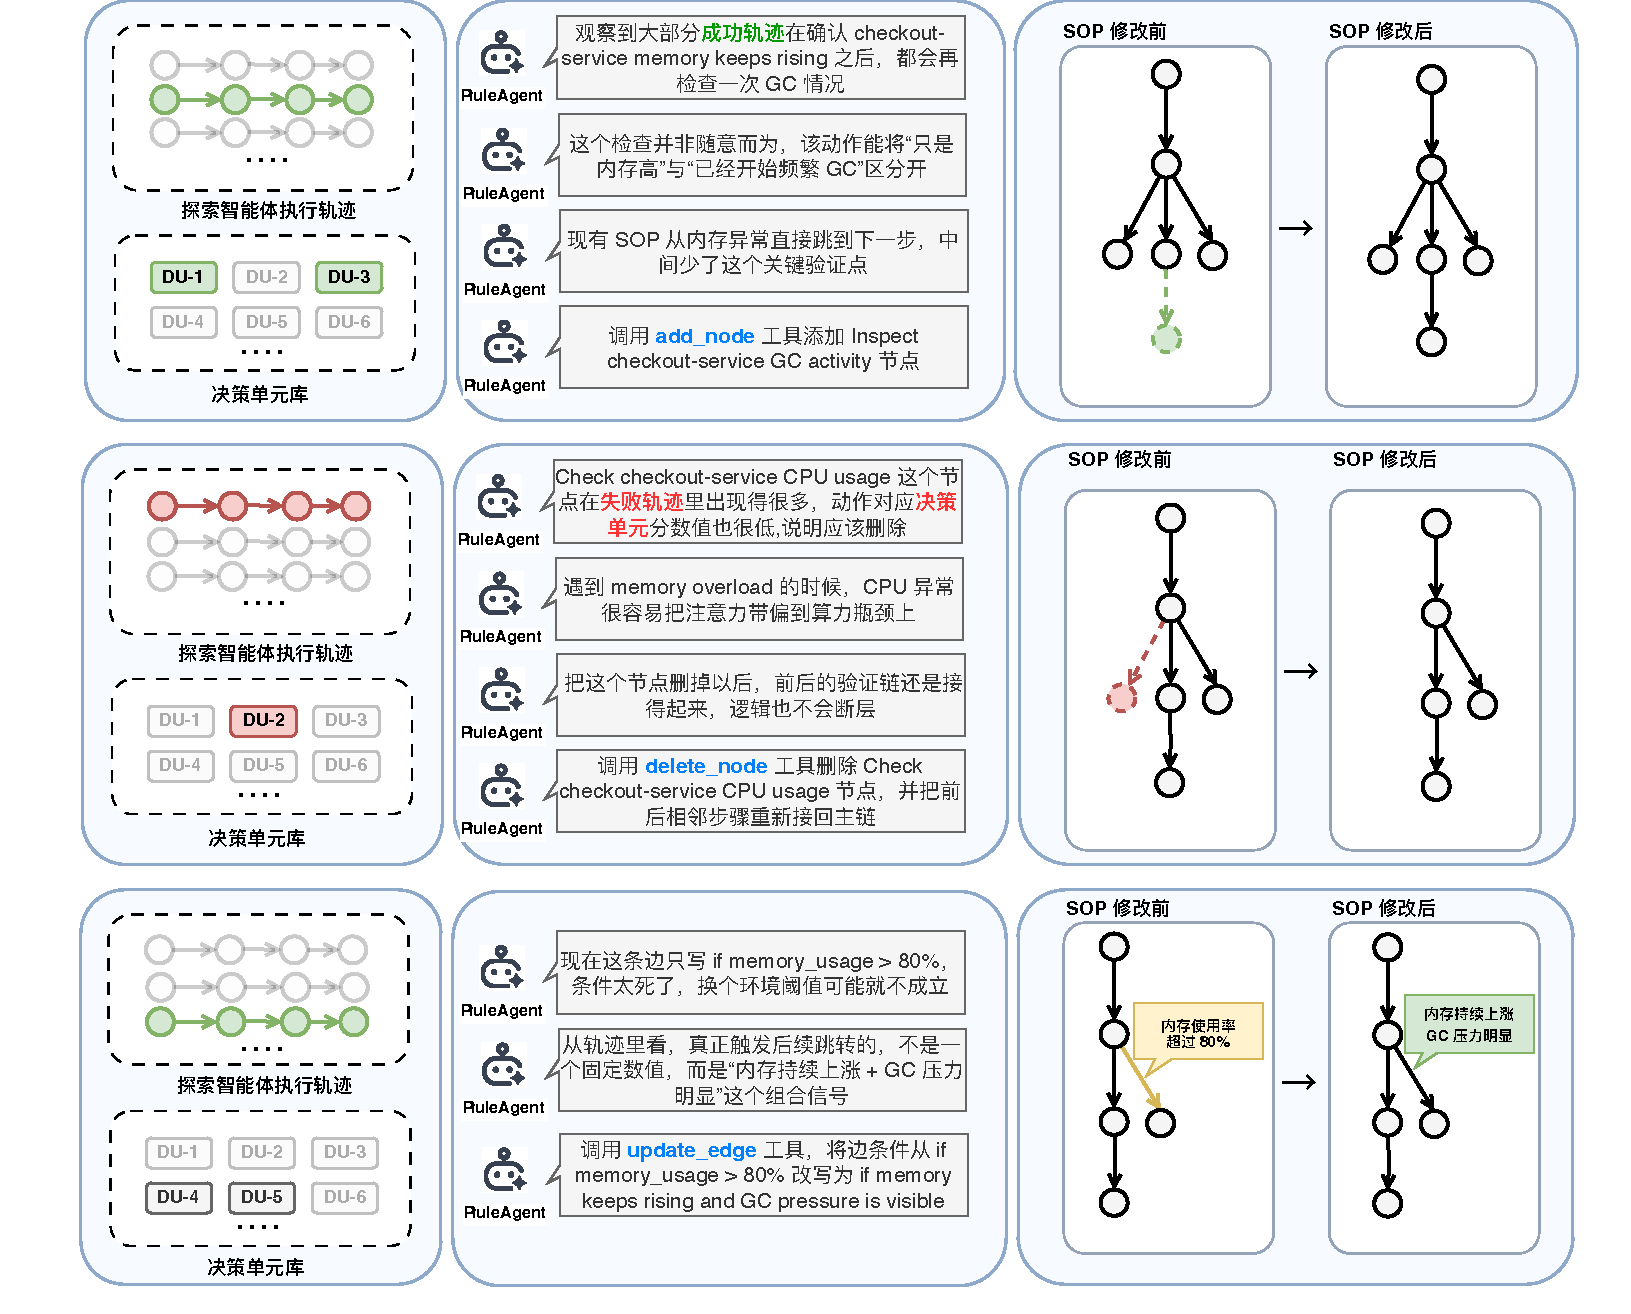
\includegraphics[width=\textwidth]{Figures-Src/Chap3-Methodology/sop-construction-case/chart.pdf}
    \bicaption{\enspace 执行轨迹构建SOP的示意}{\enspace Illustration of SOP Construction from Execution Trajectories}
    \label{fig:sop_rule}
\end{figure}

结合图\ref{fig:sop_rule}，RuleAgent 对 SOP 的组织主要体现在三类操作上：添加、删除和修改。

\begin{enumerate}[label=（\arabic*）]
    \item \textbf{添加：把当前 SOP 中缺失、但已被多次验证有效的检查步骤补入原有路径。}图\ref{fig:sop_rule}上半部分给出了一个新增节点的例子。多条成功轨迹表明，在确认 \texttt{checkout-service} 内存持续升高之后，诊断过程通常还会继续检查一次 GC 状态；而现有 SOP 在“内存异常”之后直接跳转到下一步，中间缺少这一检查节点。RuleAgent 在对照轨迹时，会先从当前 SOP 中定位到“内存异常”所在节点，再结合带权决策单元库判断“检查 GC 情况”是否属于反复出现且有效的局部判断。若答案为是，则调用 \texttt{add\_node} 与 \texttt{add\_edge}，把 \texttt{Inspect checkout-service GC activity} 作为新的中间节点插入原路径中。新增的不是一条临时轨迹片段，而是一个已经被多次成功执行支持的缺失步骤。

    \item \textbf{删除：把长期误导诊断、且在失败路径中频繁出现的步骤从 SOP 中移除。}图\ref{fig:sop_rule}中间部分展示了一个删除节点的例子。节点“\texttt{Check checkout-service CPU usage}”在失败轨迹中出现频繁，而对应决策单元的权重也较低，说明该检查步骤虽然经常被执行，但并没有稳定帮助诊断收敛。在内存过载场景下，这一步往往把排查方向过早引向 CPU 瓶颈，造成注意力偏移。RuleAgent 在读取全部已标记轨迹后，会发现该节点更多出现在未能收敛的路径中，并且删除该节点后，前后的验证关系仍然可以自然衔接。因此，它会调用 \texttt{delete\_node} 或 \texttt{delete\_edge}，将这一低价值步骤从当前 SOP 中移除，并把前后相邻节点重新接回主链。删除的依据不是“这一步出现次数少”，而是“这一步反复出现，但对正确定位根因没有形成稳定贡献”。

    \item \textbf{修改：保留原有节点或边，但把过于僵硬或不准确的表达改写为更符合真实诊断规律的条件。}图\ref{fig:sop_rule}下半部分对应的是条件修改。旧版本 SOP 只写“\texttt{if memory\_usage > 80\%}”，这类固定阈值便于书写，但与真实诊断过程并不完全一致。轨迹显示，真正触发后续排查的并不是某个孤立的数值点，而是“内存持续上升，同时伴随明显 GC 压力”的组合信号。RuleAgent 在比较多条执行轨迹后，会发现当“内存持续升高 + GC 压力明显”出现时，后续路径具有更高的一致性，而单独的“超过 80\%”并不能稳定区分是否需要继续下钻。因此，它不会删除该分支，而是调用 \texttt{update\_edge}，把原来的边条件改写为更贴近真实触发模式的表达。修改保留了原有结构，但提升了 SOP 条件语义的准确性。
\end{enumerate}

这三类操作分别对应补足缺失步骤、清理误导路径和修正触发条件。随着同类故障实例不断积累，这些局部更新会反复发生，因此 SOP 的形成本质上是一个持续校正和逐步补全的过程。

为了使上述编辑可追踪、可回滚，RuleAgent 的行为被限制在一组智能体工具之内。表\ref{tab:ruleagent_tools}给出了 RuleAgent 在组织 SOP 时使用的工具集合。

\begin{table}[tbp]
    \centering
    \bicaption{\enspace 规则智能体的 SOP 组织工具}{\enspace Tools Used by RuleAgent for SOP Organization}
    \label{tab:ruleagent_tools}
    \renewcommand{\arraystretch}{1.25}
    \fontsize{10pt}{12pt}\selectfont
    \setlength{\tabcolsep}{3pt}
    \begin{tabular*}{\textwidth}{@{\extracolsep{\fill}}>{\centering\arraybackslash}p{2.0cm}>{\centering\arraybackslash}p{1.9cm}>{\raggedright\arraybackslash}p{5.2cm}>{\raggedright\arraybackslash}p{4.0cm}@{}}
        \toprule
        \rowcolor{lightgray!30}
        \textbf{工具类别} & \textbf{工具名称} & \textbf{功能描述} & \textbf{关键参数} \\
        \midrule
        \multirow{3}{*}{\textbf{知识读取}}
        & \texttt{get\_decision\_unit} & 读取当前故障类型的带权决策单元及统计信息 & fault-type \\
        \cline{2-4}
        & \texttt{read\_trajectory} & 读取当前故障类型的已标记执行轨迹及上下文证据 & fault-type, label, batch-size \\
        \cline{2-4}
        & \texttt{read\_sop} & 读取当前版本 SOP 的节点、边及版本信息 & sop-id, version \\
        \midrule
        \multirow{7}{*}{\textbf{SOP 局部更新}}
        & \texttt{add\_node} & 插入新的诊断动作节点 & parent-node-id, intent, entity \\
        \cline{2-4}
        & \texttt{add\_edge} & 添加条件跳转关系 & source-node-id, target-node-id, condition \\
        \cline{2-4}
        & \texttt{update\_node} & 更新节点意图或实体表达 & node-id, intent, entity \\
        \cline{2-4}
        & \texttt{update\_edge} & 更新边条件或约束语义 & edge-id, condition \\
        \cline{2-4}
        & \texttt{delete\_node} & 删除无效或重复节点 & node-id \\
        \cline{2-4}
        & \texttt{delete\_edge} & 删除无效跳转关系 & edge-id \\
        \cline{2-4}
        & \texttt{save\_sop} & 保存 SOP 版本及更新说明 & sop-id, version-note \\
        \bottomrule
    \end{tabular*}
    \setlength{\tabcolsep}{6pt}
\end{table}

经过上述组织后，系统得到的不是脱离旧版本重新生成的一张新图，而是在当前版本 SOP 上完成的一次局部更新结果。一次故障实例可能只暴露出一个缺失节点，也可能只说明某条旧路径应被删除，或者只推动某个条件表达被改写；当同类故障不断出现时，这些局部写回会持续累积到同一份 SOP 上，使其中的诊断知识被一步一步提取出来。最终得到的 SOP 仍表示为有向无环图，并与对应故障簇建立绑定关系，供后续在线诊断阶段直接召回与执行。
